\section{Specifica del problema e modello realizzativo del progetto}
Nel momento in cui mi trovo a scrivere e parlare di questo mio progetto, milioni di utenti stanno visualizzando in giro per il mondo una mappa, che sia essa su Google, Bing o proveniente dal database di OSM. Molti sviluppatori, allo stesso tempo, stanno strutturando al meglio un qualsiasi generico sistema che, utilizzando le stesse mappe, permetta di collocare su di esse oggetti, informazioni e molti altri dati.

Uno dei problemi forse maggiori è la poca flessibilità offerta da questi servizi. Infatti, sfruttando ad esempio alcune funzioni presenti in CSS 3, è possibile prendere la stessa mappa interattiva di Google, inserirla all'interno del body della pagina HTML, ed ottenere una vista semi-prospettica. Il risultato però non appare altrettanto nitido e pulito come accade con una canvas tridimensionale. La mappa, infatti, in questo contesto verrebbe schiacciata in altezza più che stampata lungo un ipotetico terzo asse di riferimento. Proprio per questo motivo, creare un sistema che mostri le mappe del mondo in una vista prospettica, permette la consultazione delle stesse e, ad esempio, un loro utilizzo più attivo, rispetto ad una semplice visualizzazione. Come si può vedere nella figura \ref{fig:rotationcss}, modificando in CSS il parametro "transform" con attributo "rotateX(50deg)" il risultato è di gran lunga lontano dalla sua idea di visualizzazione.

\begin{figure}[H]
	\centering
	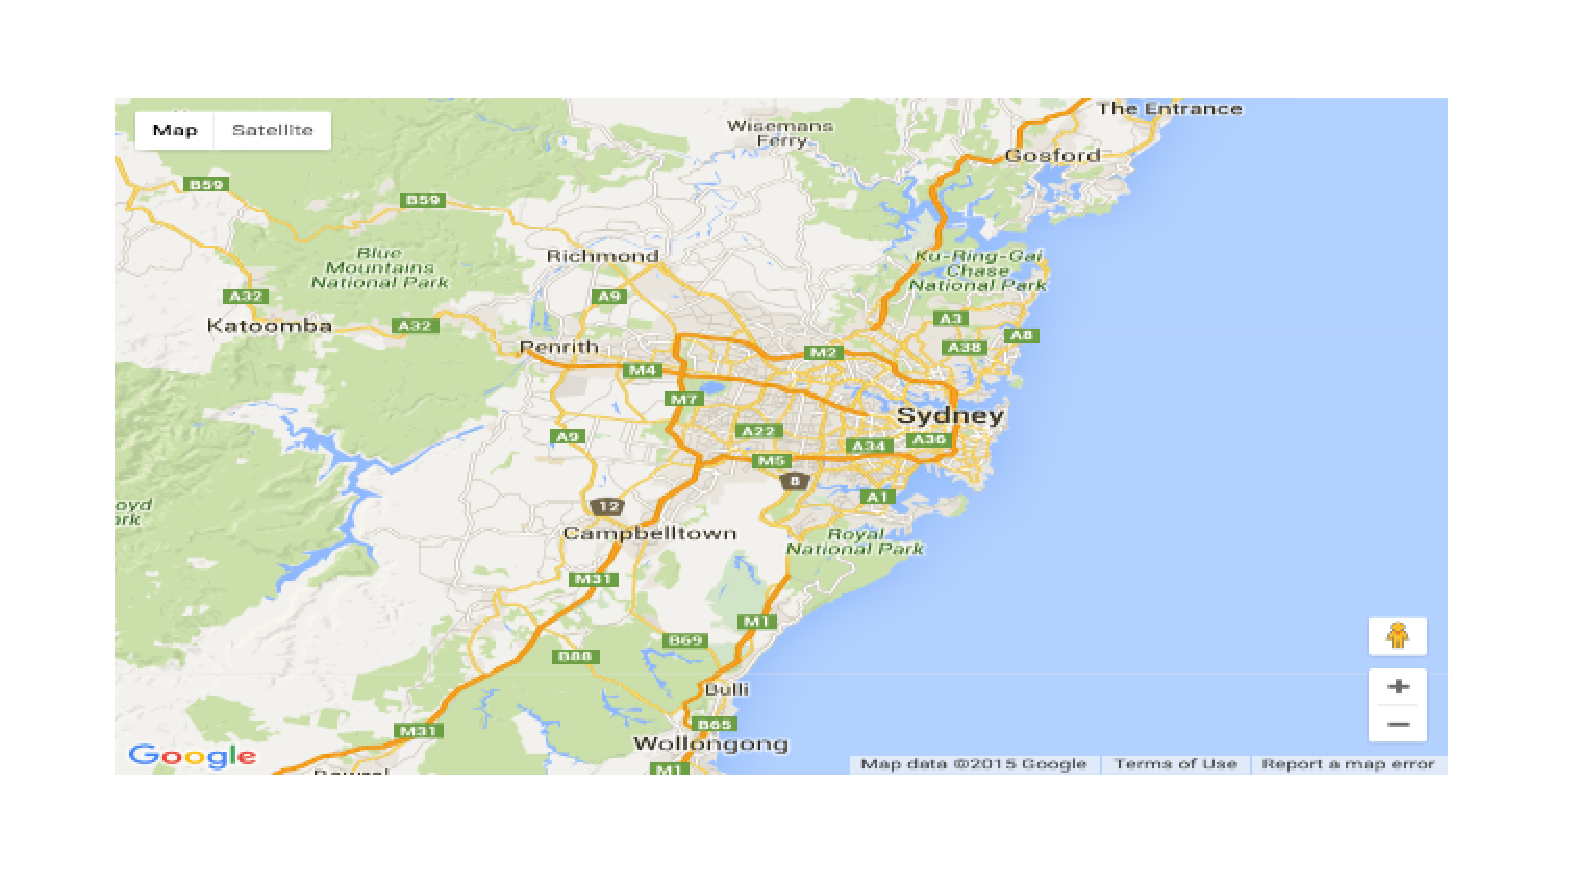
\includegraphics[scale=0.5]{figure/rotationcss.eps}
	\caption{Esempio di mappa con angolo di visualizzazione editato nel CSS}\label{fig:rotationcss}
\end{figure}

Non essendo, dunque, CSS 3 la soluzione migliore da applicare, si è deciso di utilizzare Three.js per la realizzazione di questo sistema. Attraverso l'utilizzo di questa libreria è stato possibile oltre alla renderizzazione della mappa su un piano prospettico, anche la realizzazione di un sistema che consenta all'utente una completa interazione con esso. Sarà possibile dunque, utilizzando la tastiera, navigare letteralmente sulle mappe, potendo muoversi e zoomare su di esse.

Utilizzando sempre \textit{Google Maps} come esempio, la stessa società di Mountain View permette all'interno delle sue mappe di effettuare un "tilt" sul layer, ovvero ruotare rispetto all'asse x la visualizzazione della mappa. La struttura, però, di questa funzione è molto complessa. Essendo disponibile solo per le mappe satellitari, oltre a rappresentare le mappe e le strade permette di visualizzare anche le diverse altitudini dei terreni e una rappresentazione tridimensionale degli edifici come è possibile vedere nella figura \ref{fig:tiltmap}.

\begin{figure}[H]
	\centering
	\includegraphics[scale=0.5]{figure/tiltmap.eps}
	\caption{Esempio della funzione tilt sul polo della Vasca Navale}\label{fig:tiltmap}
\end{figure}

Uno dei punti di forza del progetto, la cui architettura completa analizzerò nel corso del prossimo capitolo, è sicuramente il fatto che le mappe non vengono scaricate e/o collezionate in alcun database, ma esse stesse vengono richieste direttamente dalla sorgente (Google Maps) e caricate sul nostro client, in un diretto streaming del flusso di dati. Il fatto di non dover memorizzare tutte le mappe, oltre ad essere un vantaggio economico, di risparmio dal punto di vista delle componenti effettivamente necessarie, pemette anche di mantenere sempre aggiornate le stesse informazioni non dovendo  periodicamente controllare la presenza di modifiche sui dati presenti nello stesso database.

Questo progetto potrebbe, infine, essere la base di partenza per molti altri casi di studio. Molto spesso, ad esempio, si vorrebbe disegnare la topografia di una rete conoscendo le cordinate o gli indirizzi delle macchine che ne fanno parte. Grazie a questo sistema di visualizzazione, si avrebbe una veduta d'insieme maggiore rispetto a quella che probabilmente avremmo posizionando dei semplici "pin" all'interno di una mappa di Google.